\begin{figure}[t]
\centering
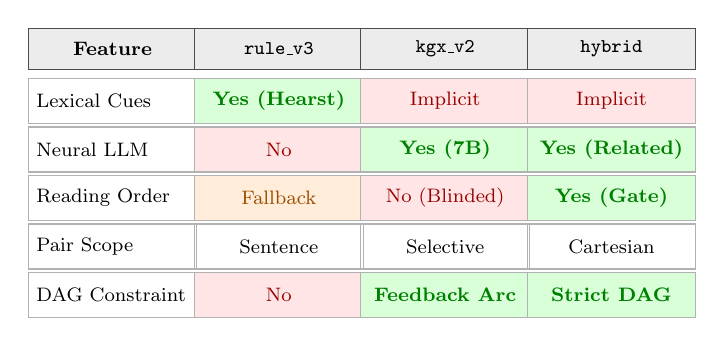
\begin{tikzpicture}[
    scale=0.88, every node/.style={transform shape, font=\footnotesize},
    header/.style={rectangle, draw=black!70, fill=gray!15, text width=2.2cm, align=center, font=\footnotesize\bfseries, minimum height=0.6cm},
    cell/.style={rectangle, draw=black!30, text width=2.2cm, align=center, minimum height=0.65cm},
    yesnode/.style={cell, fill=green!15, text=green!50!black, font=\footnotesize\bfseries},
    nonode/.style={cell, fill=red!10, text=red!60!black},
    partnode/.style={cell, fill=orange!15, text=orange!60!black}
]

% Headers
\node[header] (h0) at (0,0) {Feature};
\node[header] (h1) at (2.4,0) {\texttt{rule\_v3}};
\node[header] (h2) at (4.8,0) {\texttt{kgx\_v2}};
\node[header] (h3) at (7.2,0) {\texttt{hybrid}};

% Row 1: Explicit Cues
\node[cell, align=left] (r10) at (0,-0.75) {Lexical Cues};
\node[yesnode] (r11) at (2.4,-0.75) {Yes (Hearst)};
\node[nonode] (r12) at (4.8,-0.75) {Implicit};
\node[nonode] (r13) at (7.2,-0.75) {Implicit};

% Row 2: Neural Semantics
\node[cell, align=left] (r20) at (0,-1.45) {Neural LLM};
\node[nonode] (r21) at (2.4,-1.45) {No};
\node[yesnode] (r22) at (4.8,-1.45) {Yes (7B)};
\node[yesnode] (r23) at (7.2,-1.45) {Yes (Related)};

% Row 3: Reading Order
\node[cell, align=left] (r30) at (0,-2.15) {Reading Order};
\node[partnode] (r31) at (2.4,-2.15) {Fallback};
\node[nonode] (r32) at (4.8,-2.15) {No (Blinded)};
\node[yesnode] (r33) at (7.2,-2.15) {Yes (Gate)};

% Row 4: Candidate Pairing
\node[cell, align=left] (r40) at (0,-2.85) {Pair Scope};
\node[cell] (r41) at (2.4,-2.85) {Sentence};
\node[cell] (r42) at (4.8,-2.85) {Selective};
\node[cell] (r43) at (7.2,-2.85) {Cartesian};

% Row 5: Graph Constraints
\node[cell, align=left] (r50) at (0,-3.55) {DAG Constraint};
\node[nonode] (r51) at (2.4,-3.55) {No};
\node[yesnode] (r52) at (4.8,-3.55) {Feedback Arc};
\node[yesnode] (r53) at (7.2,-3.55) {Strict DAG};

\end{tikzpicture}
\caption{Information sources and inductive constraints across the three construction pipelines.}
\label{fig:methodology_comparison}
\end{figure}
